\documentclass[]{report}
\usepackage[table,xcdraw]{xcolor}
\usepackage{graphicx}
\usepackage{geometry}
\usepackage[utf8x]{inputenc}
\usepackage{lmodern,textcomp}
\pdfminorversion=5 
\pdfcompresslevel=9
\pdfobjcompresslevel=2
\geometry{legalpaper, margin=0.6in}
\graphicspath{ {./imgs/} }

\title{PROGRAMA DO CONCURSO POR SORTEIO \\ ARRENDAMENTODE HABITAÇÕES ARENDAS ACESSÍVEIS \\ ~\\ $[$II$]$ \\}
\author{pela Porto Vivo, SRU -Sociedade de Reabilitação Urbana do Porto, E.M., S.A.}
\date{02.2020}

\begin{document}

\maketitle

%\section*{}

\pagenumbering{gobble}



\begin{table}[]
	\begin{center}
	\begin{huge}
	\begin{tabular}{c}
		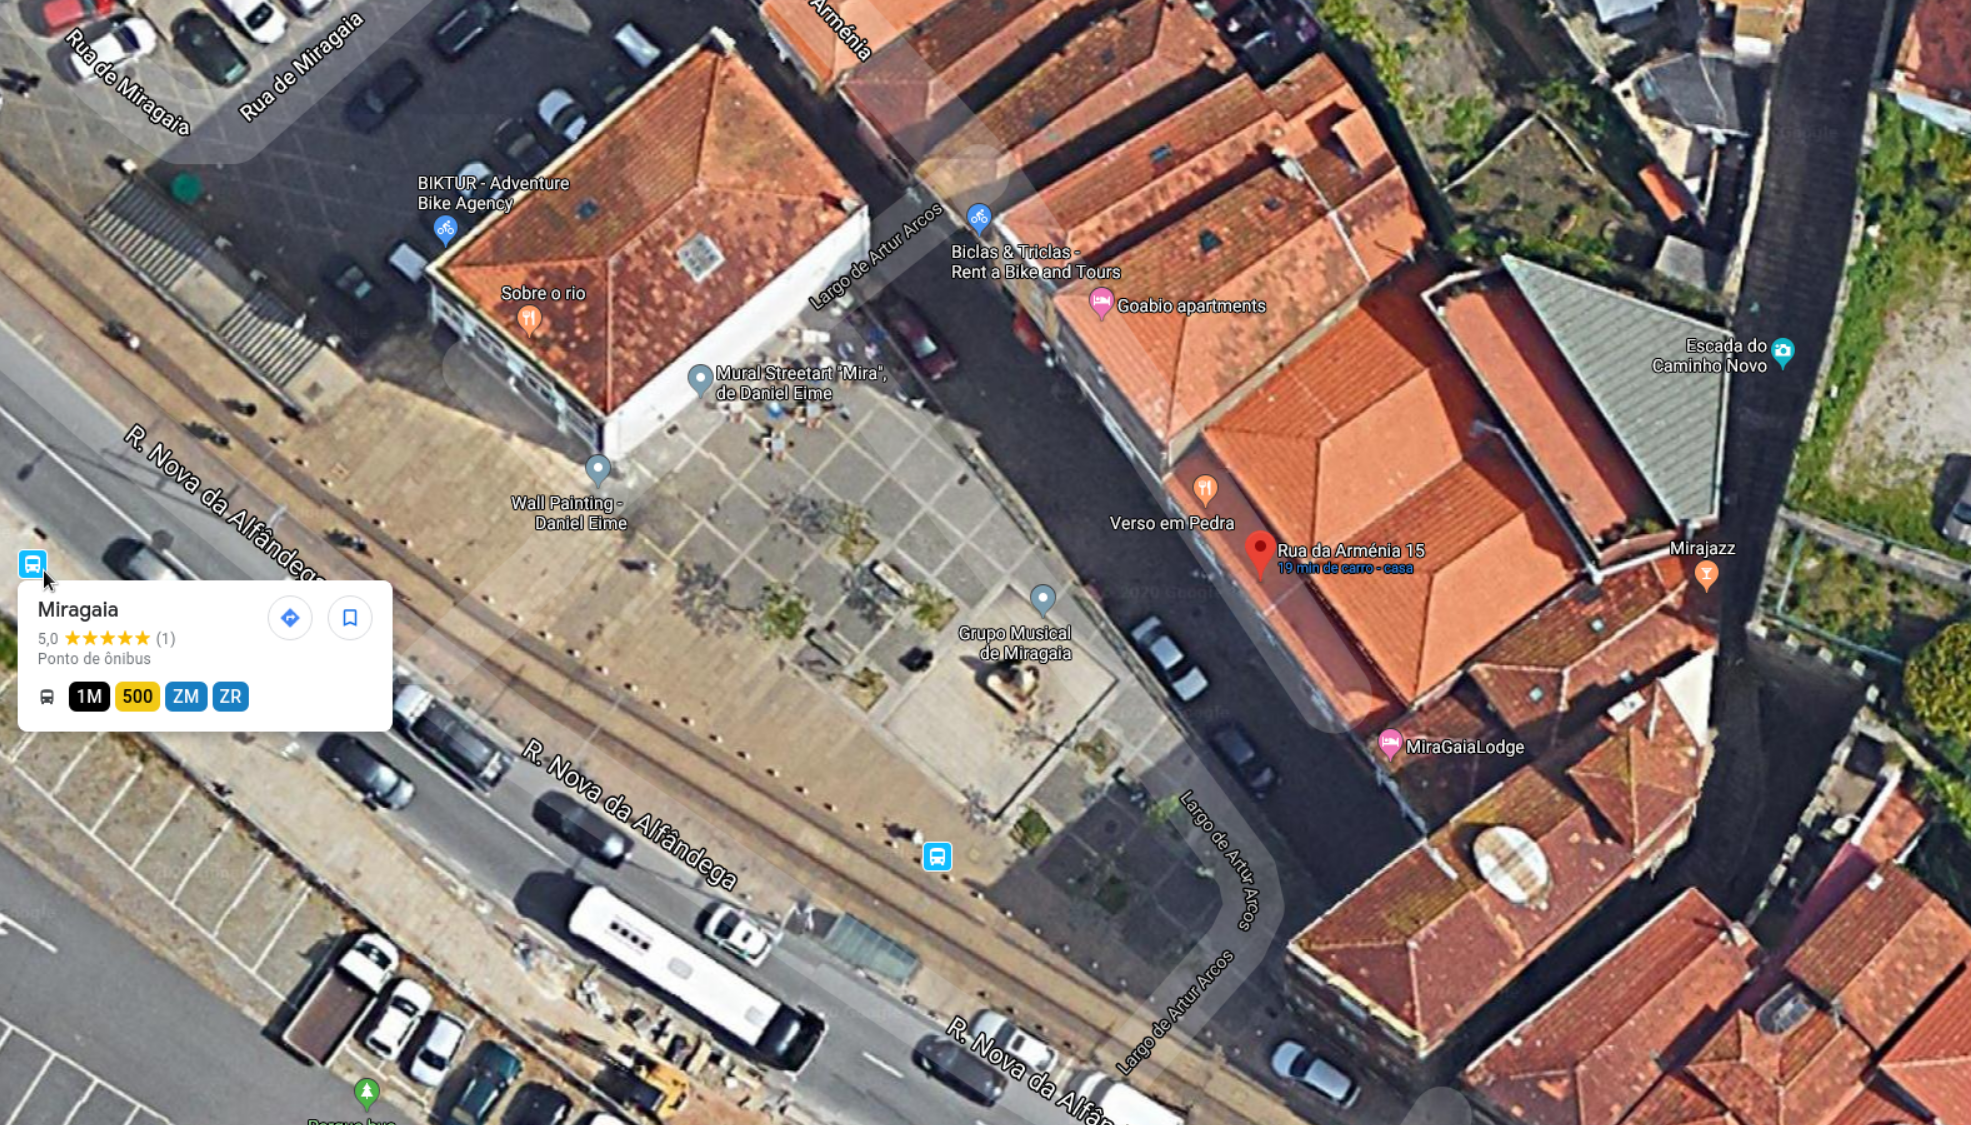
\includegraphics[width=1\textwidth]{rua_da_armenia_n_15_rc_sat} \\
		~\\
		~\\
		~\\
		~\\
		~\\
		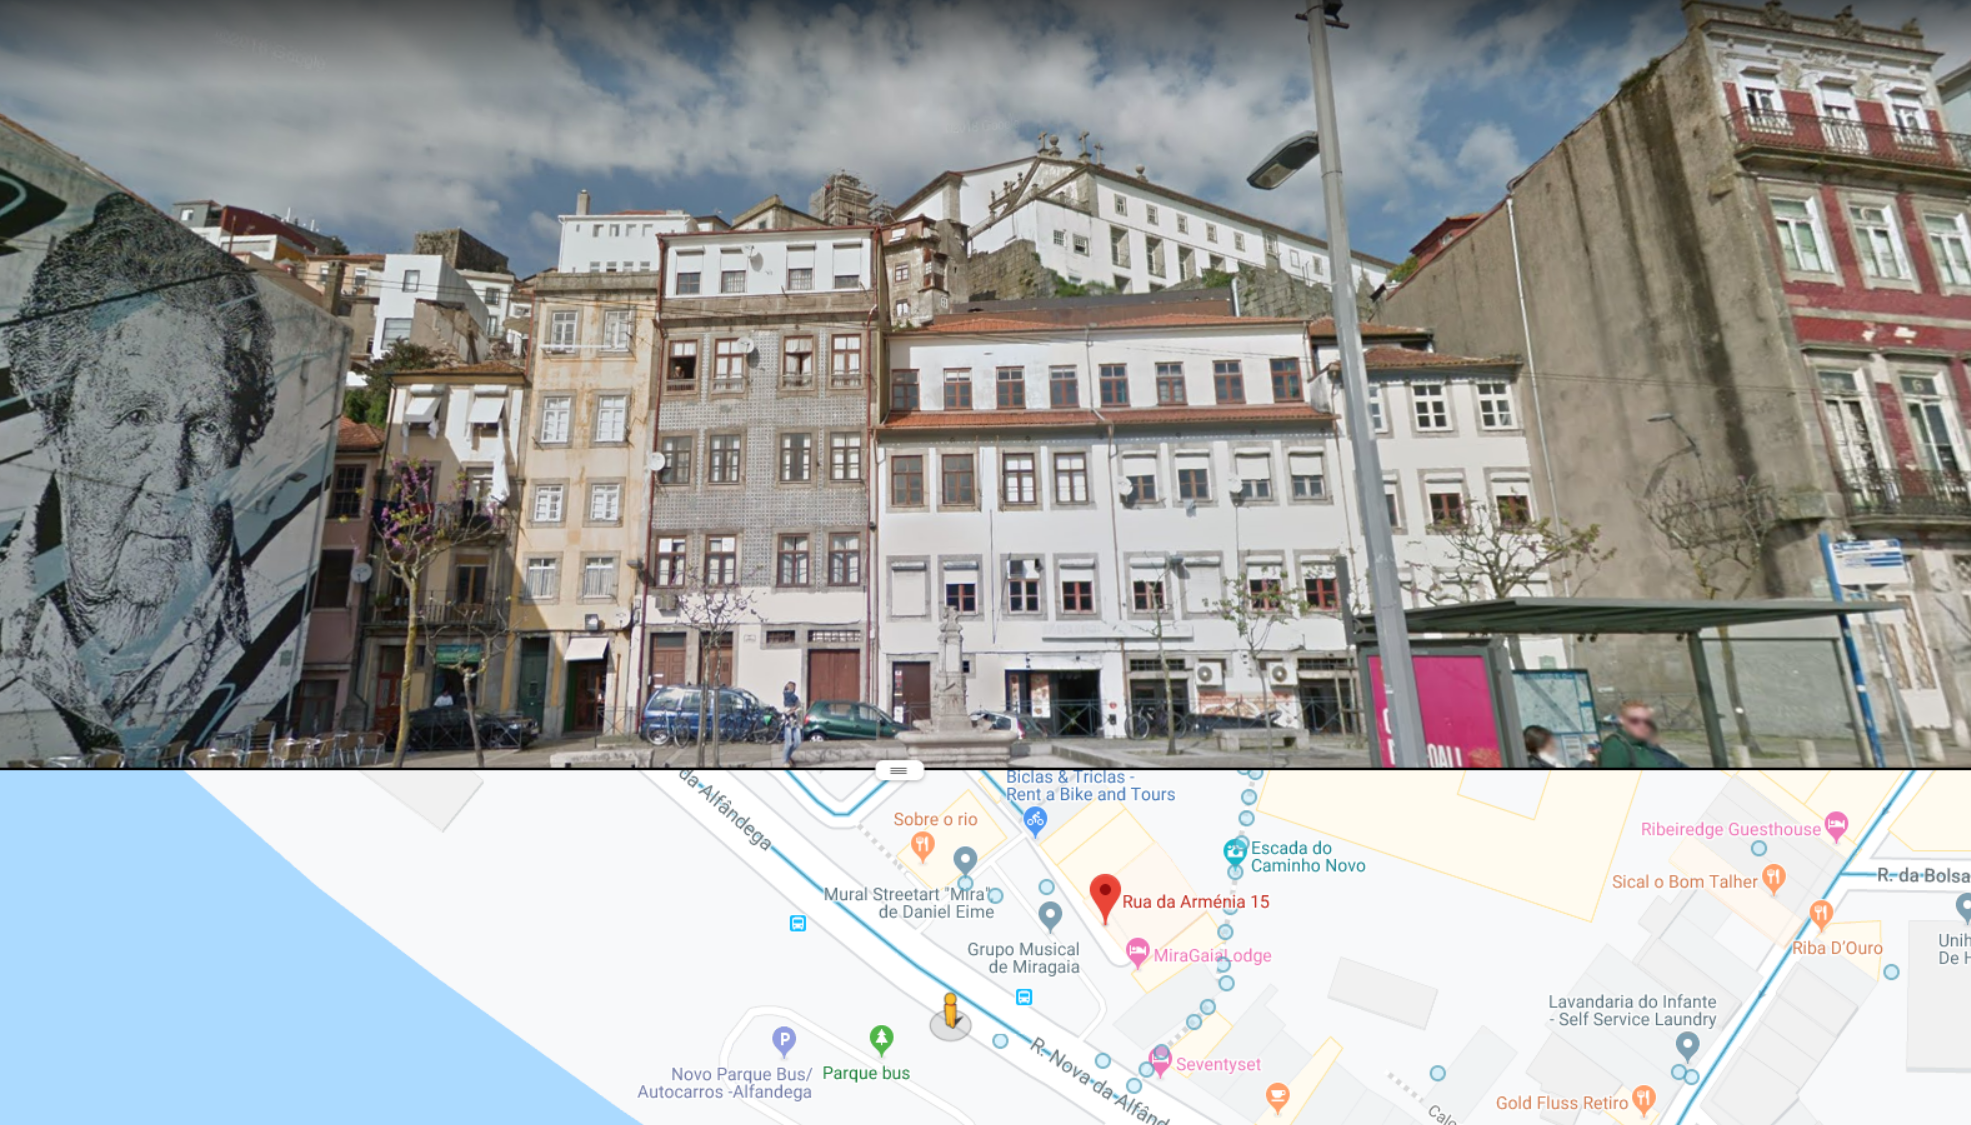
\includegraphics[width=1\textwidth]{rua_da_armenia_n_15_rc_str} \\
		~\\
		~\\
		~\\
		~\\
		~\\
		\textcolor{gray}{T0, Rua da Arm\'{e}nia, 15, R/C [247,23€] (48$m^{2}$)}
	\end{tabular}
	\end{huge}
	\end{center}
\end{table}

\begin{table}[]
	\begin{center}
	\begin{huge}
	\begin{tabular}{c}
		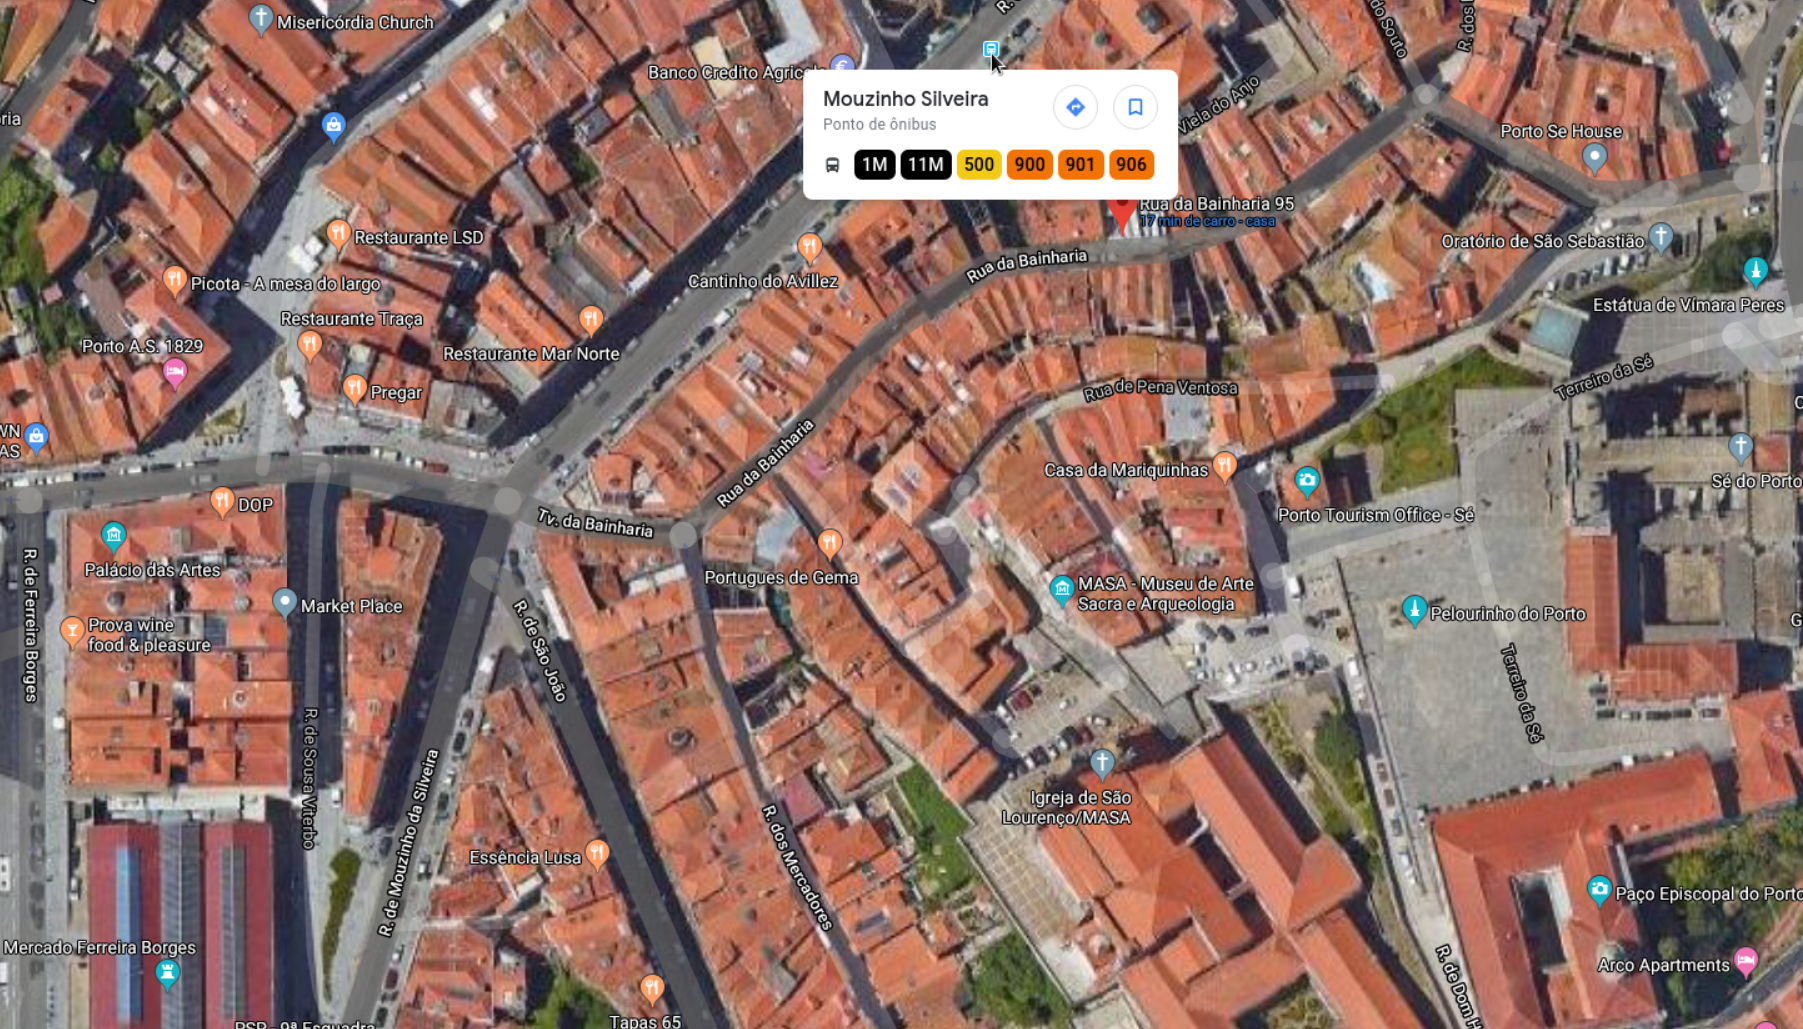
\includegraphics[width=1\textwidth]{rua_da_bainharia_95_97_rc_sat} \\
		~\\
		~\\
		~\\
		~\\
		~\\
		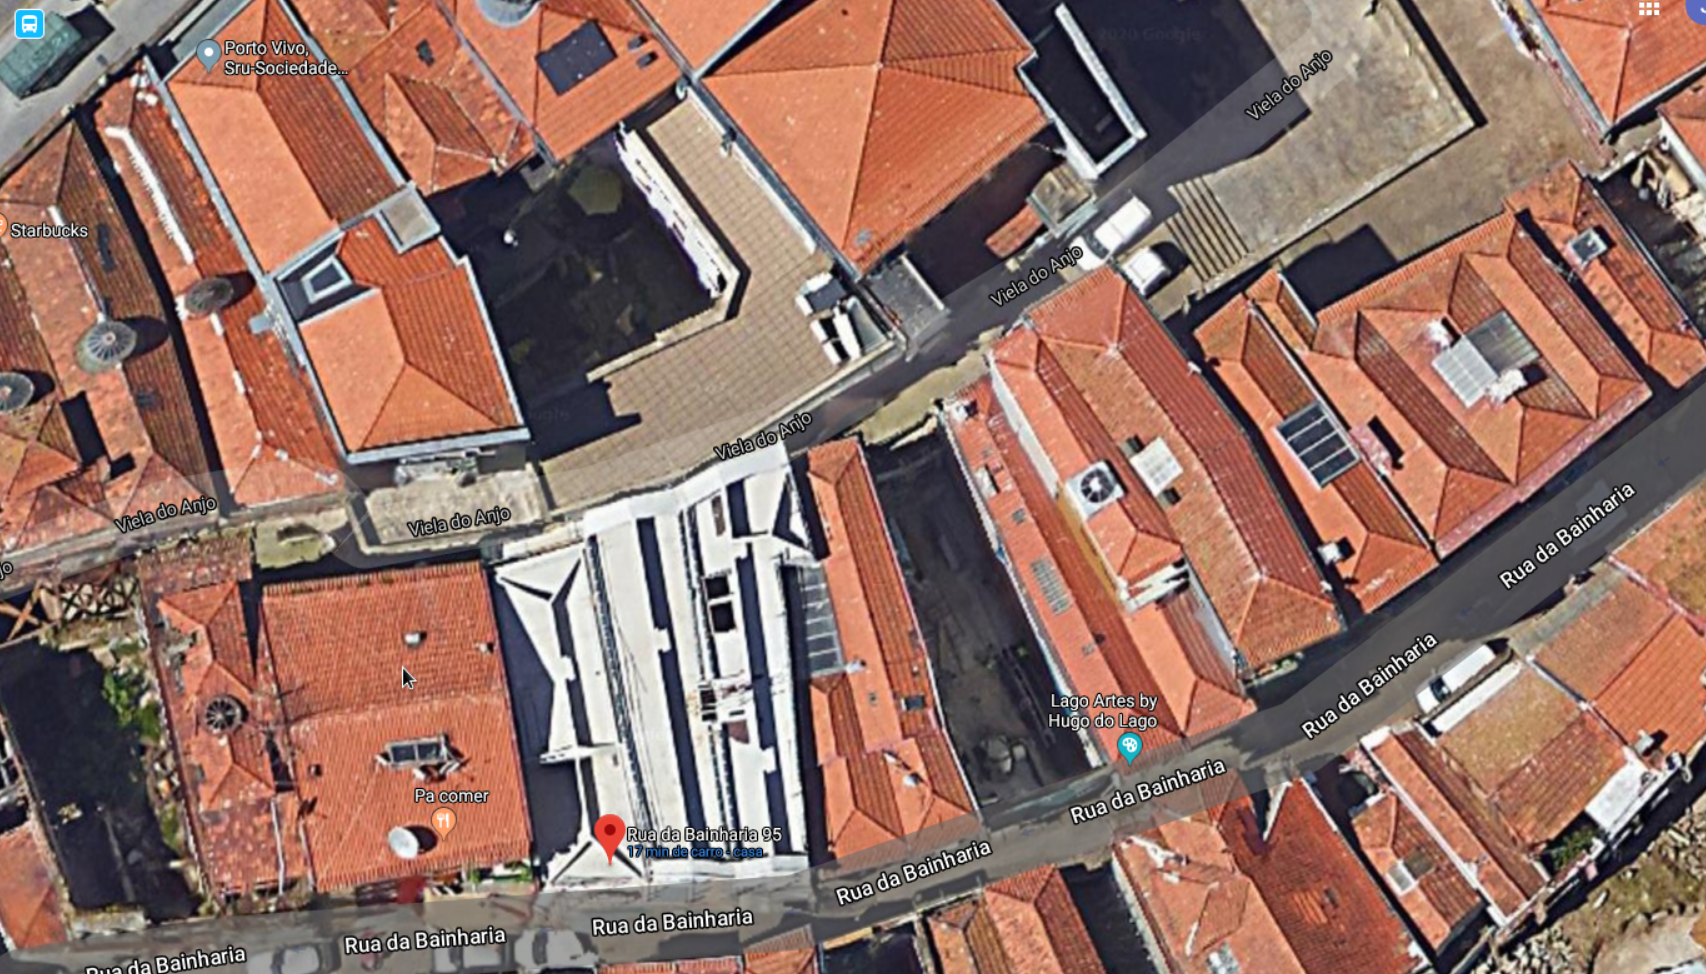
\includegraphics[width=1\textwidth]{rua_da_bainharia_95_97_rc_str} \\
		~\\
		~\\
		~\\
		~\\
		~\\
		\textcolor{gray}{T0, Rua da Bainharia, 95/97, R/C [227,47€] (52$m^{2}$)}
	\end{tabular}
	\end{huge}
	\end{center}
\end{table}

\begin{table}[]
	\begin{center}
	\begin{huge}
	\begin{tabular}{c}
		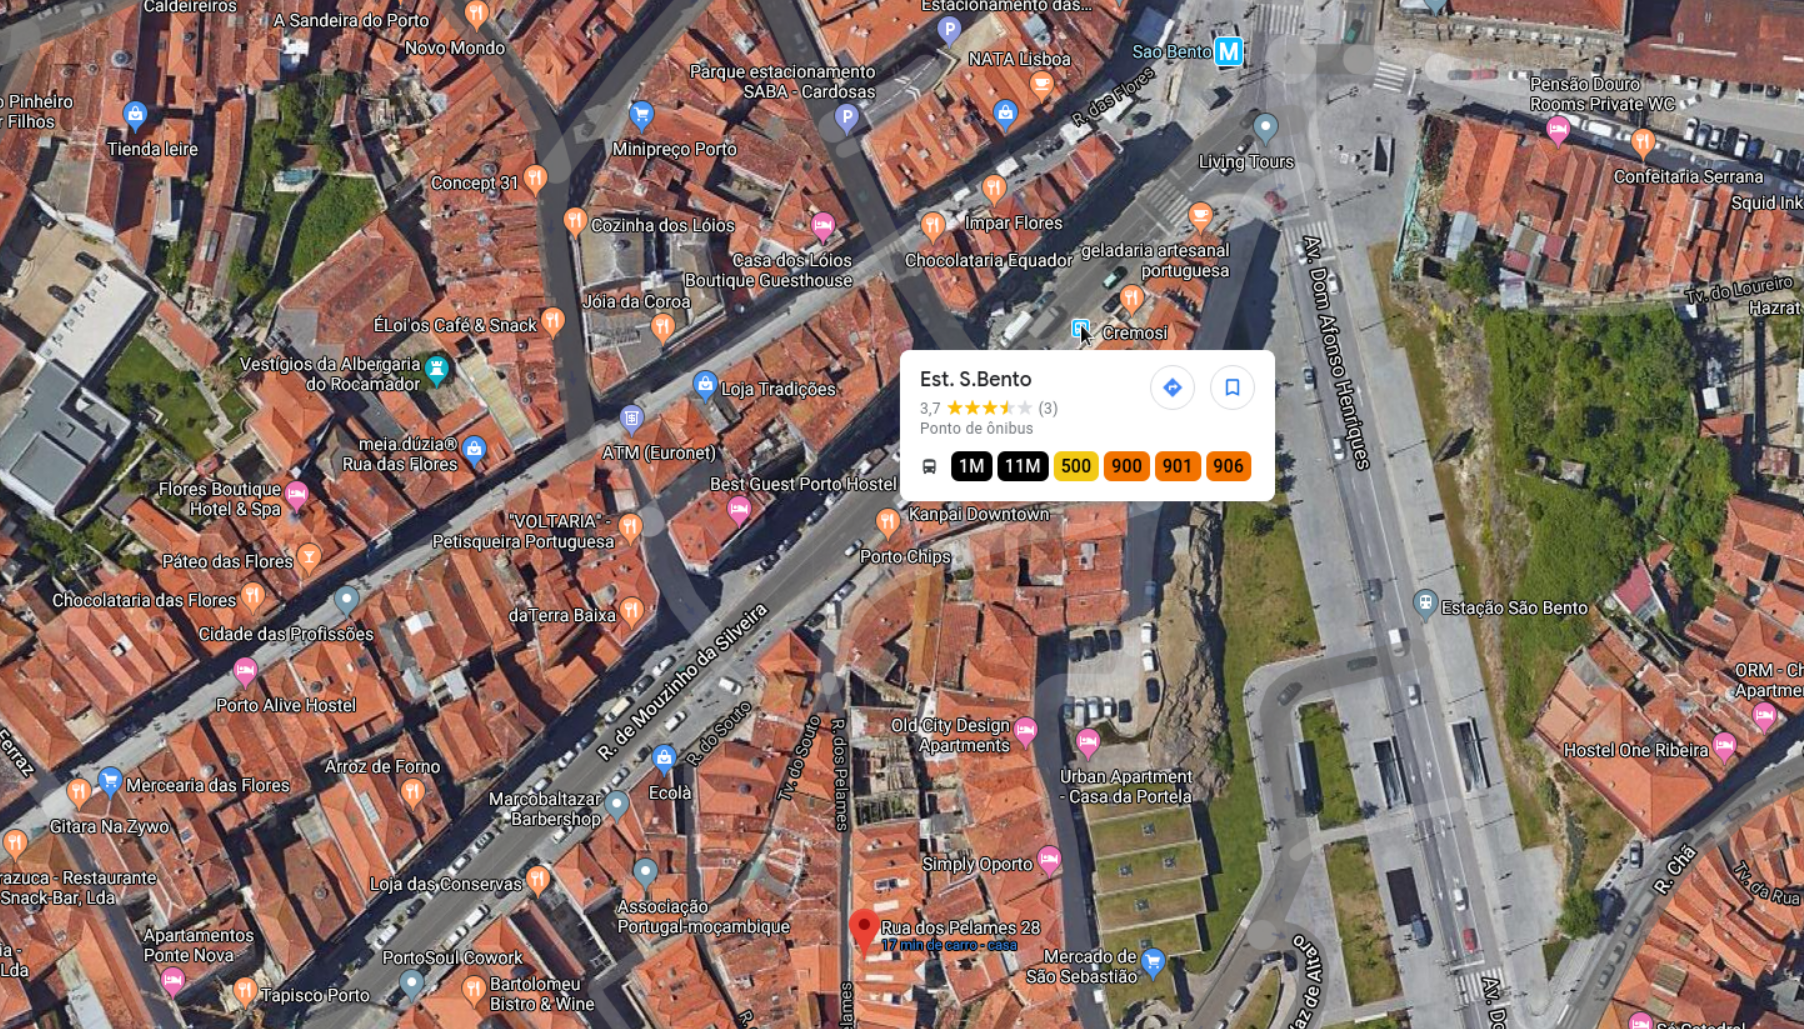
\includegraphics[width=1\textwidth]{rua_dos_pelames_28_rc_sat} \\
		~\\
		~\\
		~\\
		~\\
		~\\
		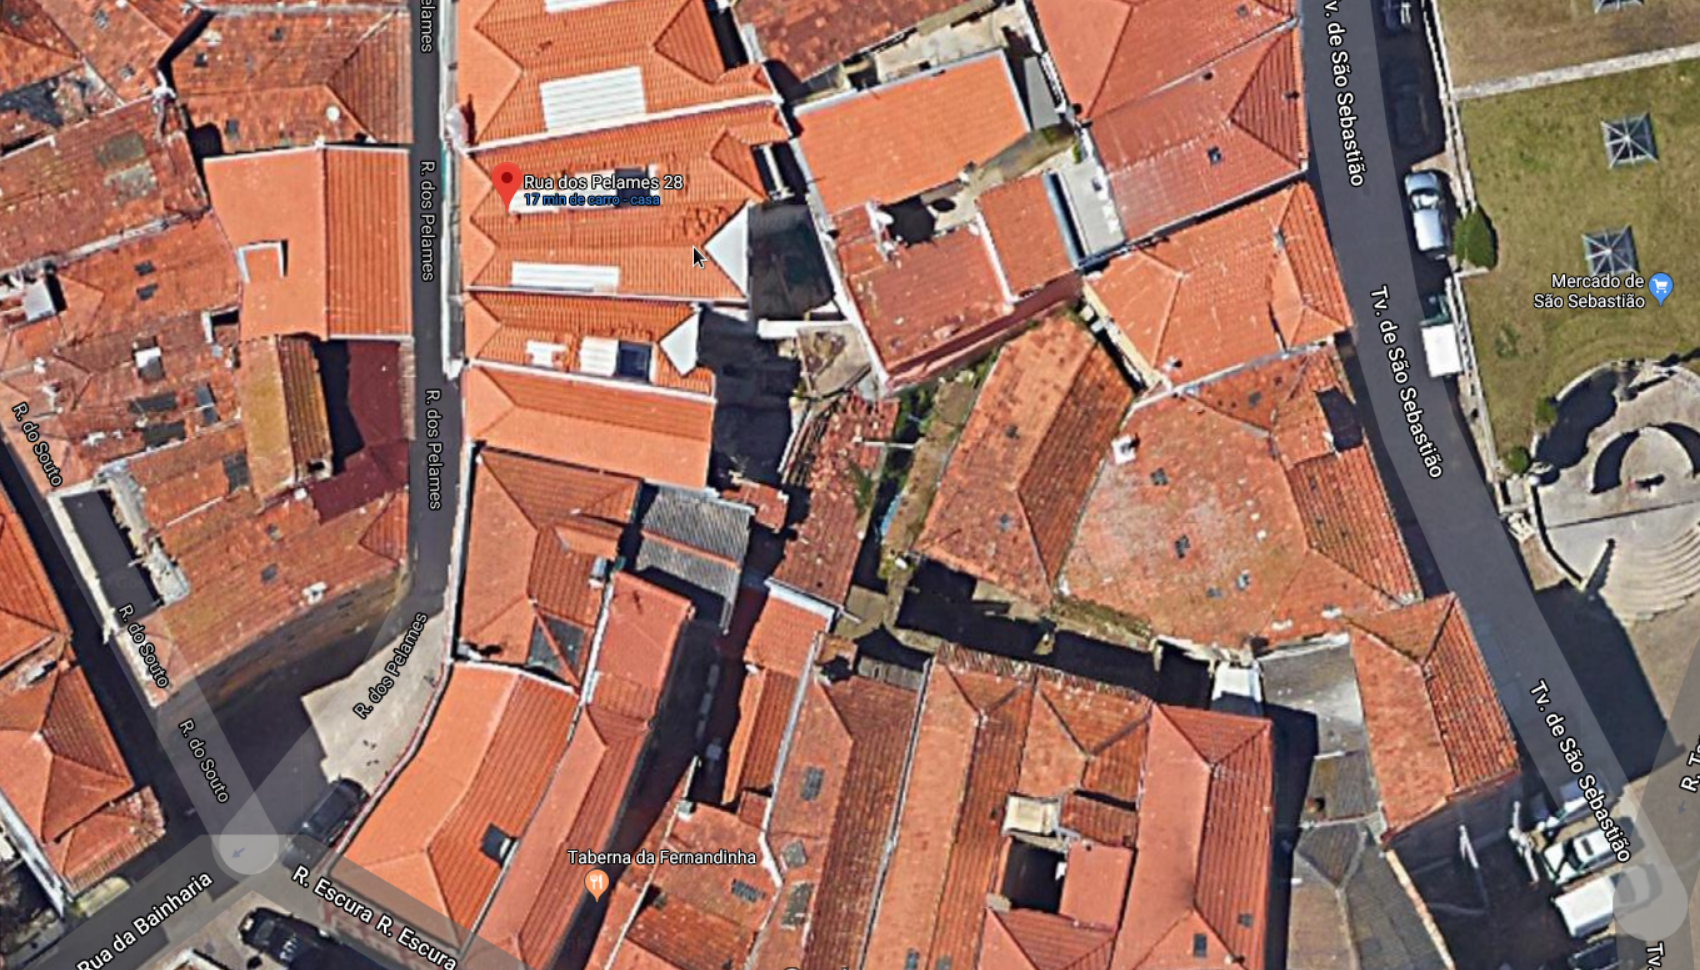
\includegraphics[width=1\textwidth]{rua_dos_pelames_28_rc_str} \\
		~\\
		~\\
		~\\
		~\\
		~\\
		\textcolor{gray}{T0+1, Rua dos Pelames, 28, R/C [232,49€] (53$m^{2}$)}
	\end{tabular}
	\end{huge}
	\end{center}
\end{table}


\end{document}
